\subsection{Umfrage Dashbaord}
\label{ssec:UmfrageDashboard}

Wie zuvor in Kapitel \myRefGeneral{ssec:UmfrageErstellen} dargestellt, ist das Herzstück der Applikation das Erstellen einer Umfrage. 
Nachdem der Benutzer eine Survey angelegt hat, findet dieser diese auf dieser Seite wieder.

\abb \myRefGeneral{fig:SurveyMasterDashboard} zeigt das \emph{Survey Dashboard}.
Der Benutzer kann hier über ein Suchleiste, die auch als Dropdown-Menü fungiert, seine erstellten Umfragen filtern. \newline
Die erste Karte auf dieser Seite ist von ihrem Aufbau her differenziert. Über den Button \jinline|Create New Survey Master| auf der Karte mit dem Icon \faPlusSquare, kann der Benutzer eine neue Umfrage \engl{Survey} anlegen (siehe Kap. \vref{ssec:UmfrageErstellen}). \newline
Die anderen Karten folgen einem gleichen Muster: 
\begin{itemize}
	\item Sie beinhalten immer die Anzahl der erstellten (published) Umfragen.
	\item Eine Survey kann immer über das Icon \faCopy\xspace kopiert werden. 
	Hierbei werden alle Fragen übernommen und erweitert werden. 
\end{itemize}
%
Generell unterscheiden sich die Umfragen wie folgt:
%
% \begin{itemize}
% 	\item Survey-Template erstellt und noch keine Umfrage erstellt.
% 	\item Survey-Template erstellt und mindestens eine Umfrage erstellt.
% \end{itemize}
%
\subsubsection*{Survey-Template -- keine Umfrage erstellt}
%
Der Benutzer hat die Möglichkeit, im Falle einer Falscheingabe über das Icon \faEdit\xspace wieder in den Editierungsmodus zu gelangen (vgl. \vref{ssec:UmfrageErstellen}).
Über das Icon \faTrash\xspace lässt sich die erstellte Umfrage wieder löschen, da es hierzu noch keine gestartete Umfrage gibt. 

\subsubsection*{Survey-Template -- mindestens eine Umfrage erstellt}
%
Da die Umfrage bereits gestartet ist, enfallen nun die Icons \faTrash\xspace (löschen) und \faEdit\xspace (editieren).
Als ein alleinstellungsmerkmal hat der Benutzer nun die Möglichkeit über das Icon \faIdCard\xspace zu seinen Ergebnissen zu kommen (vgl. \vref{ssec:ResultDashboardImplement}).

\begin{figure}[!htb]
	\centering
	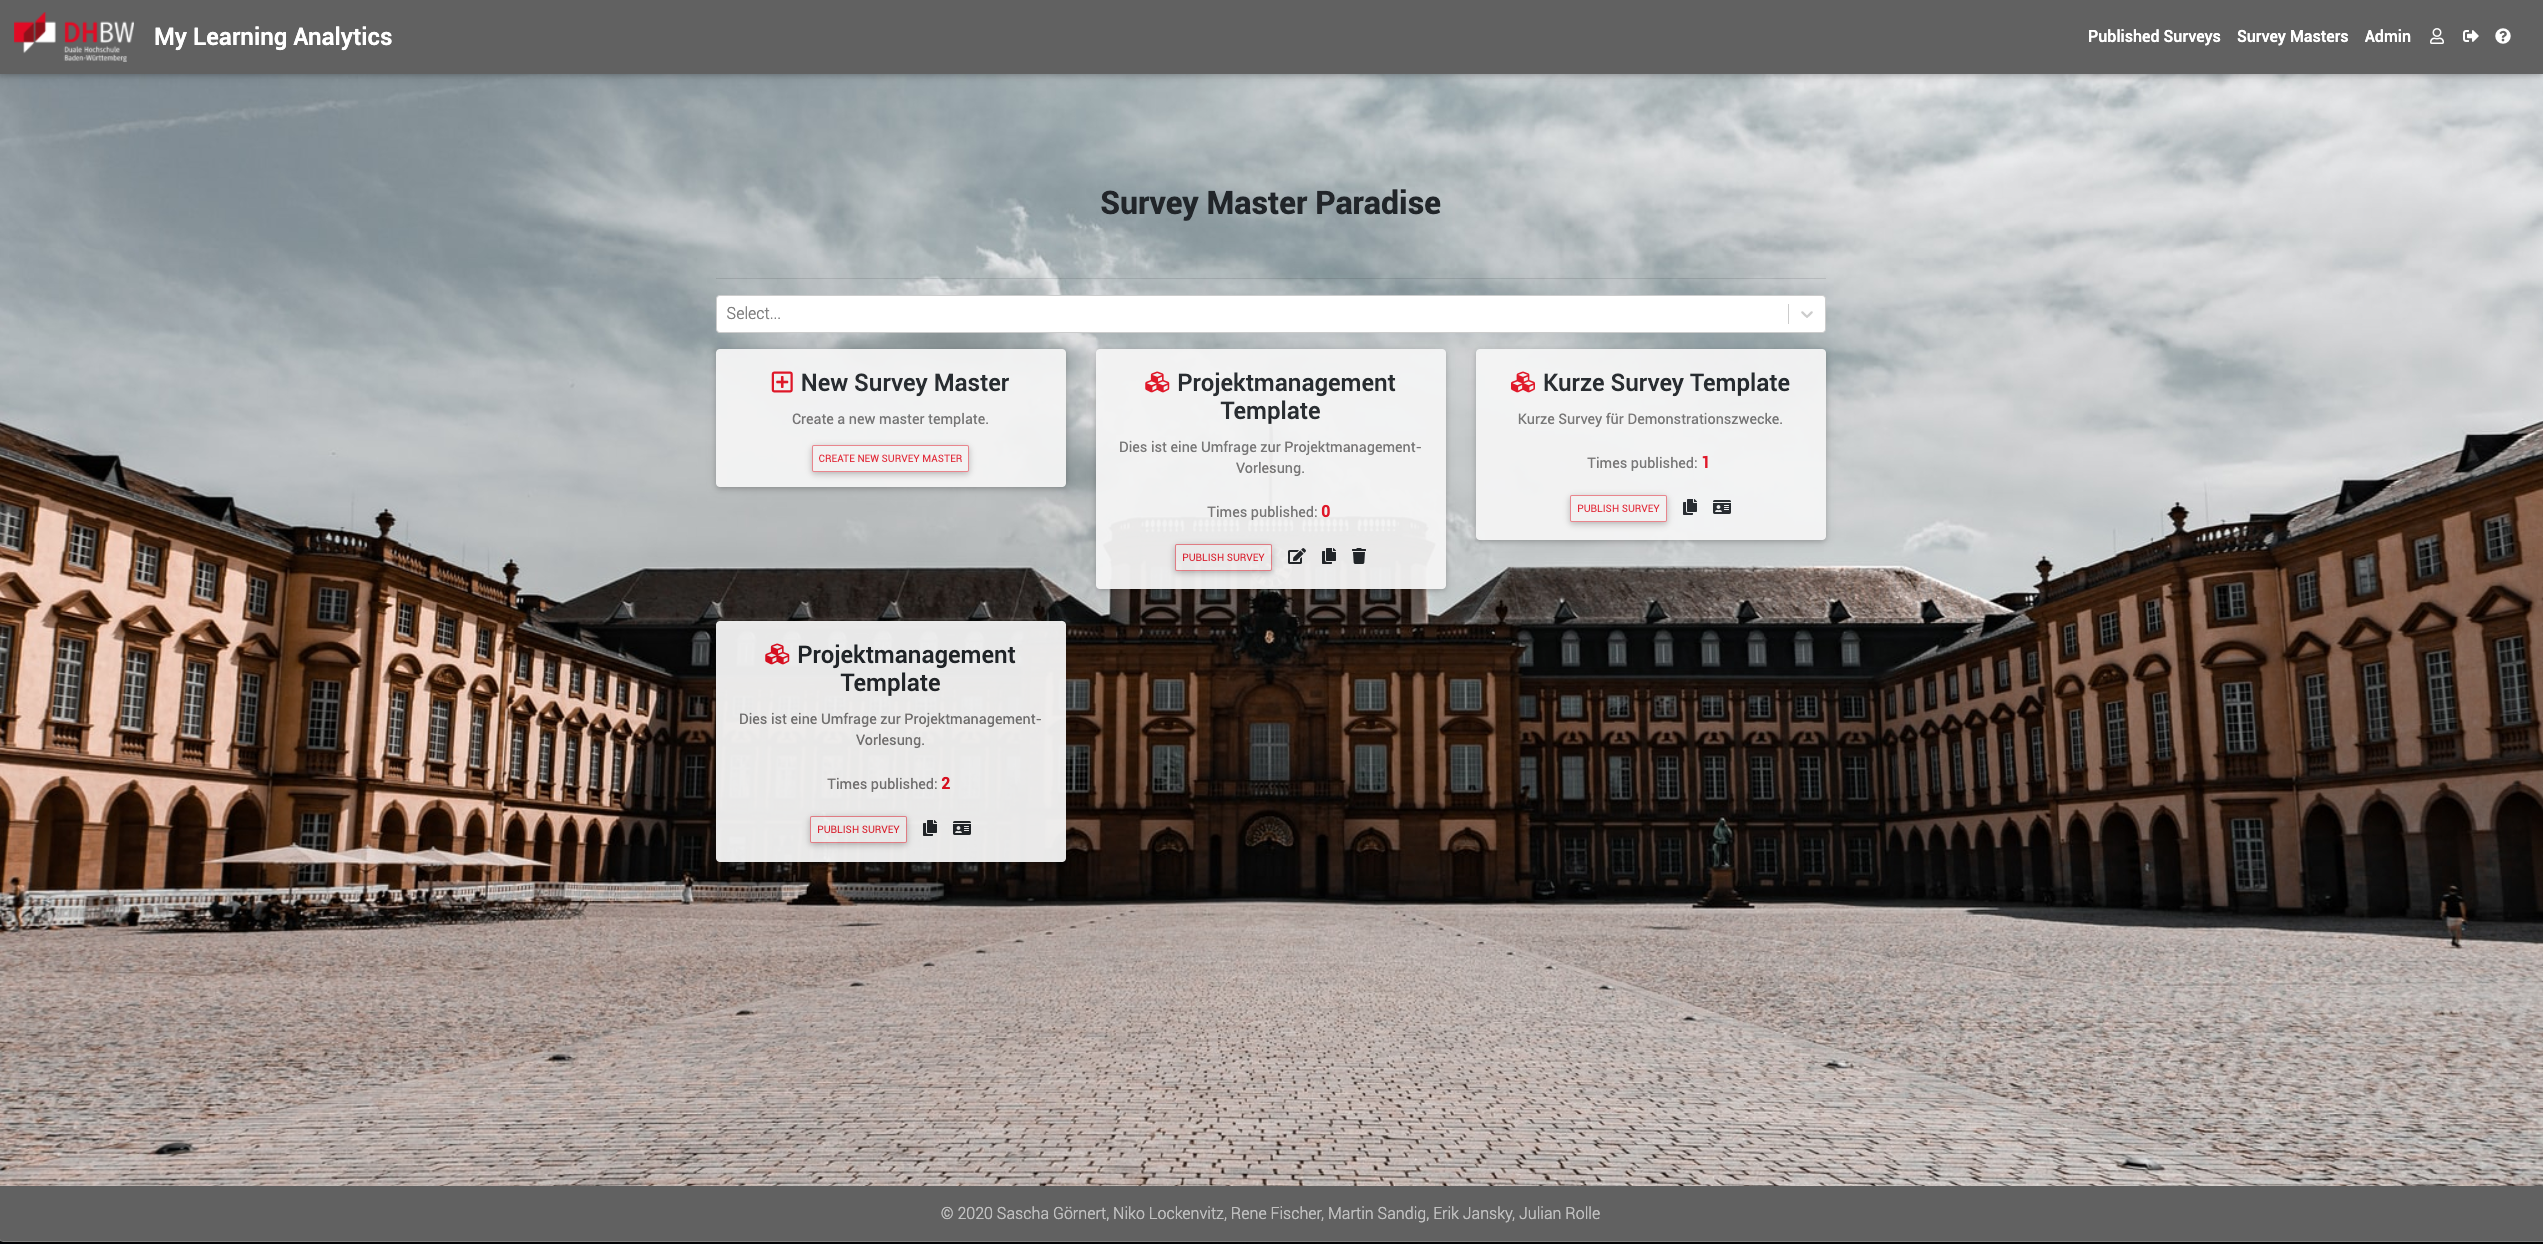
\includegraphics[width=0.95\textwidth, keepaspectratio]{img/client/SurveyMaster.png}
	\captionsetup{justification=centering, format=plain}
	\caption[\acf{UI}: Survey Dashboard]{\acf{UI}: Survey Dashboard \\ \quelleScreenshot}
	\label{fig:SurveyMasterDashboard}
\end{figure}